\documentclass[a4paper, 12pt]{report}

% Packages
\usepackage[utf8]{inputenc}
\usepackage{amsmath}
\usepackage{amsfonts}
\usepackage{amssymb}
\usepackage{graphicx}
\usepackage[backend=biber, style=numeric, sorting=nyt]{biblatex}

% Bibliography file
\addbibresource{../../literature/references.bib}

% Title and Author
\title{My Minimal Report}
\author{Your Name}
\date{\today}

\begin{document}

% Title Page
\maketitle

% Abstract
\begin{abstract}
This is a brief summary of the report. It provides an overview of the main points and findings.
\end{abstract}

% Sections
\chapter{Introduction}
This is the introduction section. Here you can introduce the topic of your report and provide some background information.

\begin{figure}[htbp]
    \centering
    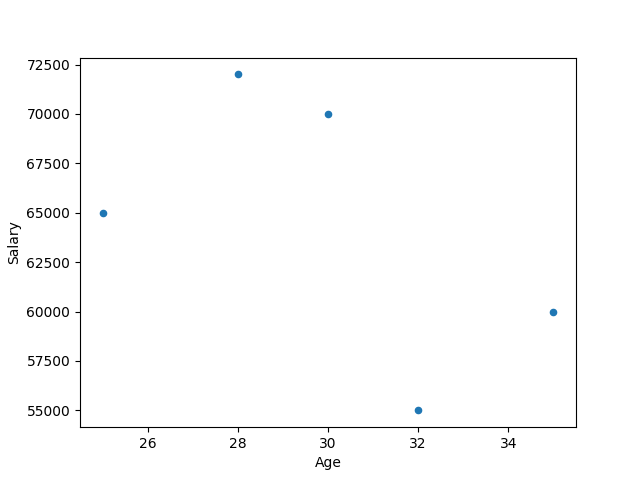
\includegraphics[width=1.0\textwidth]{../figures/demo.png}
    \caption{Caption of the figure.}
    \label{fig:examplebook}
\end{figure}

An example citation \cite{examplebook}

\chapter{Methodology}
Describe the methods and procedures used in your research or study.

\chapter{Results}
Present the results of your research or study. Use figures and tables as necessary.

\chapter{Discussion}
Discuss the implications of your results and compare them with previous research. Highlight any limitations and suggest future research directions.

\chapter{Conclusion}
Summarize the main findings of your report and their significance.

% References
\printbibliography

\end{document}